\chapter{Processamento de Linguagem Natural}
\label{cap:Processamento}

% Um computador, obviamente, está preparado para entender sua própria linguagem,
% como por exemplo, um compilador interpreta linhas de código fonte para gerar um
% programa executável seguindo exatamente o algoritmo utilizado. Por isso, temos o
% termo Natural no Processamento de Linguagem. 

O objetivo da área de Processamento de Linguagem Natural é analisar a linguagem natural, ou seja, a linguagem utilizada pelo seres humanos não
importando se essa é escrita ou falada \cite{manningschutze1999}.

O Processamento de Linguagem Natural é uma área antiga, sendo anterior a
invenção dos computadores modernos. De fato, sua primeira grande aplicação foi
um dicionário desenvolvido no Birkbeck College em Londres no ano de 1948. Por ser
uma área complexa, seus primeiros trabalhos foram notavelmente falhos o que
causou uma certa hostilidade por parte das agências formentadoras de pesquisas.

Os primeiros pesquisadores eram muitas vezes bilíngues, como por exemplo,
nativos alemães que imigraram para os Estados Unidos. Acreditava-se que pelo
fato desses terem conhecimento de ambas as linguas, Ingles e Alemão, eles teriam
capacidade de desenvolver programas de computadores que efetuariam a tradução das linguas
de modo satisfatório. Uma vez que esses encontraram muitas dificuldades,
ficou claro que o maior problema não era o conhecimento de ambas as
línguas e sim como expressar esse conhecimento na forma de um programa de
computador \cite{history}.

Para que um computador seja capaz de interpretar uma
língua, necessitamos antes entender como nós efetuamos essa
interpretação.
Por isso, uma parte considerável do Processamento de Linguagem Natural está apoiado na área de Linguística.

\section{Linguística}

O objetivo da Linguística é compreender como os humanos adquirem, produzem e
entendem as diversas línguas, ou seja, a forma com que conversamos, a nossa
escrita e outras mídias de comunicação \cite{manningschutze1999}.

Na linguagem tanto escrita, como na falada, existem regras que são utilizadas
para estruturar as expressões. Uma série de dificuldades no Processamento de
Linguagem Natural são ocasionadas pelo fato de que as pessoas constantemente
mudam essas regras para satisfazerem suas necessidades de comunicação
\cite{manningschutze1999}. Uma vez que as regras são constantemente modificadas pelo loucutor, se torna extremamente difícil a criação de um software ou hardware efetue a interpretação de uma língua. 


% \subsection{Sintaxe e Semântica}
% 
% No seu livro Estruturas Sintáticas, Noam Chomsky cita as seguintes frases
% ``Ideias verdes incolores dormem furiosamente'' e ``Incolores verde ideias dormem
% furiosamente''.
% 
% A primeira frase, do ponto de vista sintático é correta, porém, assim como a
% segunda frase, semânticamente não faz sentido.
% 
% O fato de que podemos modificar as regras da lingua de duas formas distintas é
% utilizado como evidência para a separação da sintaxe e semântica na língua.
% \cite{jacksonmoulinier2007}

\section{Métodos de Processamento de Linguagem Natural}

O \ac{NLP} tem como objetivo a execução de diferentes tarefas, como por exemplo,
a categorização de documentos, a tradução e a geração de textos a partir de um
banco de dados, etc. Podemos citar dois tipos de métodos para a execução dessas
tarefas, que são o método simbólico e o método estatístico.

Nos final dos anos 50 e 60, existiam excelentes métodos quantitativos, que foram
desenvolvidos durante a segunda guerra mundial, para a solução de problemas
científicos \cite{shannon48}.
Porém, no ano de 1957, Chomsky publicou o trabalho intitulado de
\textit{``Syntactic Structures''} e com isso, temos a primeira aparição da
teoria de gramática gerativa, que considera a gramática como um conjunto de regras. Essa abordagem através de um
conjunto de regras, ao invés de um modelo matemático, entra em conflito com os
trabalhos anteriores, criando duas comunidades no campo de Linguística. Como
reflexo das duas comunidades, a área de \ac{NLP} que crescia em paralelo a
linguística também foi dividida em duas áreas. A primeira que fazia uso de
métodos baseados em regras (simbólico) e a segunda que fazia uso de métodos
quantitativos (estatísticos).


Esta seção serão apresentados um método simbólico e um método estatístico.
Destaca-se que essa descrição apresenta como objetivo diferenciar ambos os
métodos, através de seus requisitos e forma de execução. Métodos 
utilizados na análise de sentimentos serão descritos no capítulo
\ref{cap:Classificadores}.


\subsection{Método Simbólico} 
O método simbólico ou racionalista está
baseado no campo da Linguística e faz o uso da manipulação dos símbolos,
significados e das regras de um texto. Um exemplo de método simbólico é o
método de Brill \cite{Brill:1992:SRP:974499.974526}. Por exemplo, no método de
Brill a frase ``João pintou a casa de branco'', será separada em palavras que
serão classificadas através de um dicionário pré-definido, como:

\begin{table}[htb]
\centering
\begin{tabular}{l|l|l|l|l|l|l}
Palavra         & João        & pintou & a      & casa        & de        
& branco
         \\
%Correta: & Substantivo & Verbo  & Artigo & Substantivo & Preposição &
% Substantivo \\
Classificação:   & 			   & Verbo  & Artigo & Substantivo & Preposição & Adjetivo
\end{tabular}
\label{my-label}
\end{table}

Observa-se que algumas palavras não foram
identificadas, como ``João'' ou classificadas de forma errada, como
``branco". Desta forma, o método utiliza-se de outras duas regras para uma
classificação inicial.
A primeira regra classifica todas as palavras desconhecidas que iniciam em
maiúsculo como substantivos, por exemplo, a palavra ``João''. Já a segunda regra, atribui para a palavra desconhecida a mesma classificação
de outras palavras que terminam com as mesmas três letras. Por exemplo, supondo
que a palavra ``pintou'' não fosse encontrada no dicionário, essa seria
associada a outras palavras terminadas com o sufixo ``tou''. Ou seja, essa seria
associada como verbo.

\begin{table}[htb]
\centering
\begin{tabular}{l|l|l|l|l|l|l}
Palavra         & João        & pintou & a      & casa        & de        
& branco
         \\
%Correta: & Substantivo & Verbo  & Artigo & Substantivo & Preposição &
% Substantivo \\
Classificação:   & \textbf{Substantivo} & Verbo  & Artigo & Substantivo &
Preposição & Adjetivo
\end{tabular}
\label{my-label}
\end{table}



Após essa classificação inicial, o método executa o seguinte conjunto de regras:

\begin{itemize}
   \item Se uma palavra tem a classificação \textbf{A} e está no contexto
  \textbf{C} então a sua classificação deverá ser mudada para \textbf{B}. Por
  exemplo, se uma palavra \textbf{A} (branco no exemplo) é um adjetivo e uma das
  duas palavras anteriores é uma preposição (``de'' no contexto \textbf{C}
  ), mude para sua classificação para substantivo (classificação \textbf{B}).
  
  \[\overbrace{\text{João}}^\text{Substantivo}
  \overbrace{\text{pintou}}^\text{Verbo}
  \overbrace{\text{a}}^\text{Artigo}
  \underbrace{
  \overbrace{\text{casa}}^\text{Substantivo}
  \overbrace{\text{de}}^\text{Preposição}}_\text{Contexto \textbf{C}}
  \underbrace{\overbrace{\text{branco}}^{\textcolor{red}{Adjetivo}}}_\text{Classificação
  \textbf{A}\textrightarrow\textbf{B}}
 \]
 
  \item Se uma palavra tem a classificação \textbf{A} e tem uma propriedade
  \textbf{P} então a sua classificação deverá ser alterada para \textbf{B}. Por
  exemplo, se uma palavra \textbf{A} (``Linda'') foi classificada como um
  adjetivo e é iniciada com uma letra maiúscula (propriedade \textbf{P}), sua
  classificação deverá ser alterada para substantivo (classificação \textbf{B}).
  
  \[\overbrace{\text{Comprei}}^\text{Verbo}
  \overbrace{\text{flores}}^\text{Substantivo}
  \overbrace{\text{para}}^\text{Preposição}
  \underbrace{\overbrace{\text{L}\text{inda}}^{\textcolor{red}{Adjetivo}}}_\text{Classificação
  \textbf{A}\textrightarrow\textbf{B}}
 \]
 
  \item Se uma palavra tem a classificação \textbf{A} e uma palavra com a
  propriedade \textbf{P} está na região \textbf{R}, sua classificação deverá
  ser \textbf{B}. Por exemplo, se uma das duas palavras anteriores (``João
  adora" na região \textbf{R}) iniciam com letra maiúscula (propriedade
  \textbf{P}), sua classificação deverá ser alterada para substantivo (classificação \textbf{B}).
  
   \[\underbrace{\overbrace{\text{João}}^\text{Substantivo}
  \overbrace{\text{adora}}^\text{Verbo}}_\text{Região \textbf{R}}
  \underbrace{\overbrace{\text{L}\text{inda}}^{\textcolor{red}{Adjetivo}}}_\text{Classificação
  \textbf{A}\textrightarrow\textbf{B}}
 \]
 
  
\end{itemize}

\subsection{Método Estatístico} 
O método estatístico ou empírico utiliza-se de grandes
quantidades de texto, procurando por padrões e
associações a modelos, sendo que esses podem ou não estarem relacionados com
regras sintáticas ou semânticas. 

O método estatístico para o aprendizado de máquina é considerado um
aprendizado supervisionado. Em um aprendizado supervisionado, a classificação é
feita a partir de um conjunto de dados já classificado, que é chamado de
\textit{training set}, um exemplo de método estatístico é a utilização de
Modelos de Markov com a aplicação do algoritmo de Viterbi.

Neste, a classificação da frase ``João comprou um
carro" é feita a partir de um \textit{training set} que pode, por exemplo, ser
composto de textos retirados de \textit{web-sites}, com a classe gramatical das palavras já identificada.

As palavras ``João'', ``comprou'' e ``carro''
possuem somente uma classe gramátical, sendo essa substantivo, verbo e substantivo,
respectivamente. Já a palavra ``um'' pode ser classificada em artigo (ART),
substantivo (SM) e pronome (PRO). A seguinte imagem representa
as possibilidades de caminho que o classificador pode percorrer neste exemplo:

\begin{figure}[htbp]
 \centering
 \includegraphics[height=180px]{imagens/markov.png}
 \caption{Caminhos possíveis de classificação}
 \label{fig:markov}
\end{figure}

Sendo assim, o algoritmo classificador irá utilizar o \textit{training set} para
inferir essa classificação, por exemplo, se o \textit{training set} tiver 10000 substantivos,
aonde que, 150 são a palavra ``um'' classificada como substantivo, ele irá
calcular a probabilidade da palavra ``um'' pertencer a uma determinada classe
através de:

\[ P(palavra|classe) = \frac{C(classe,palavra)}{C(classe)} \]

\[ P(um|SM) = \frac{C(SM,um)}{C(SM)} = \frac{150}{10000} = 0.015 \]

\textbf{Um} é a palavra que está sendo classificada e \textbf{SM}
são os substantivos existentes no nosso \textit{training set}. Portanto a
probabilidade de um substantivo ser associada a palavra ``um''
(\textbf{P(um$\vert$SM)}) é igual a quantidade da palavra ``um''
classificada como substantivo (\textbf{C(SM,um)}) dividida pela quantidade de
substantivos em nosso \textit{training set}.

% Para as demais palavras, serão considerados os seguintes valores:
% 


Além da probabilidade de associação a uma determinada classe, é calculada a
probabilidade de transição de uma classe para a outra. Supondo que no nosso
\textit{training set} hipotético, dos 10000 substantivos, 7000 são seguidos por
uma outra palavra classificada como verbo, essa probabilidade será calculada
através de:

\[ P(transicao|classe) = \frac{C(classe,transicao)}{C(classe)} \]

\[ P(VB|SM) = \frac{C(SM,VB)}{C(SM)} = \frac{7000}{10000} = 0.7 \]

Onde \textbf{VB} são verbos e \textbf{SM} substantivos. Como pode ser observado
na equação, a probabilidade de um substantivo ser seguido de um verbo
(\textbf{(VB$\vert$SM)}) é igual a ocorrência de substantivos seguidos de verbos (\textbf{C(SM,VB)})
dividida pela quantidade total de substantivos em nosso \textit{training set}.

A probabilidade de associação é cálculada para todas as classes e também
para todas as palavras que estão sendo classificadas, assim como a
probabilidade de transição é calculada para todas as classes. Neste, serão
considerados os seguintes valores calculados a partir do nosso \textit{training
set} de exemplo:

\begin{table}[htb]
\centering
\begin{tabular}{|l|l|l|l|l|}
\hline
            & João & comprou & um    & carro \\ \hline
Substantivo & 0.01 & 0       & 0.015 & 0.02  \\ \hline
Verbo       & 0    & 0.012   & 0     & 0     \\ \hline
Artigo      & 0    & 0       & 0.030 & 0     \\ \hline
Pronome     & 0    & 0       & 0.005 & 0     \\ \hline
\end{tabular}
\caption{Tabela de Probabilidades de Associação}
\label{tabela:associacao}
\end{table}

\begin{table}[htb]
\centering
\begin{tabular}{|l|l|l|l|l|}
\hline
            & Substantivo & Verbo & Artigo & Pronome \\ \hline
Início      & 0.30        & 0.25  & 0.35   & 0.4     \\ \hline
Substantivo & 0.4         & 0.2   & 0.015  & 0.85    \\ \hline
Verbo       & 0.5         & 0.2   & 0.3    & 0.07    \\ \hline
Artigo      & 0.1         & 0.001 & 0.030  & 0.005   \\ \hline
Pronome     & 0.7         & 0.005 & 0.005  & 0.8     \\ \hline
\end{tabular}
\caption{Tabela de Probabilidade de Transição}
\label{tabela:transicao}
\end{table} 

Para identificação do caminho correto de classificação (Figura \ref{fig:markov})
e portanto a classe gramatical da palavra ``um'', é utilizado o algoritmo de Viterbi, o qual tem o
objetivo de encontrar a sequência de eventos com mais probabilidade de ocorrer.
Começando pelo início da frase, essa sequência é calculada através de:

\[ v_t(j) = v_{t-1} a_{ij} b_j(o_t) \]

Aonde que $v_t$ é a probabilidade do caminho atual, $v_{t-1}$ é o resultado do
caminho anterior, $a_{ij}$ é a probabilidade de transição e $b_j(o_t)$ é a
probabilidade de associação.

Portanto a palavra ``João'', $v_{t-1}$ é representada pelo valor 1, visto
que essa é a primeira palavra e não foram feitos cálculos anteriores, $a_{ij}$ é
a probabilidade de transição entre ``Início'' e um substantivo, disponível na tabela \ref{tabela:transicao} e $b_j(o_t)$ é
a probabilidade de associação da palavra João com substantivo, disponível na
tabela \ref{tabela:associacao}:

\[ v_t(j) = 1 * 0.3 * 0.1 = 0.003 \]

Para ``comprou'', além dos valores retirados das tabelas \ref{tabela:transicao}
e \ref{tabela:associacao}, $v_{t-1}$ é representado pelo cálculo do
caminho anterior, ou seja, 0.003:

\[ v_t(j) = 0.003 * 0.2 * 1 = 0.0006 \] 

Ao efetuar o cálculo de todos os caminhos, para determinar qual a classificação
correta de uma palavra, é escolhido o caminho que tem maior probabilidade, no
caso apresentado, a palavra ``um'' é classificada como artigo.

\begin{figure}[htbp]
 \centering
 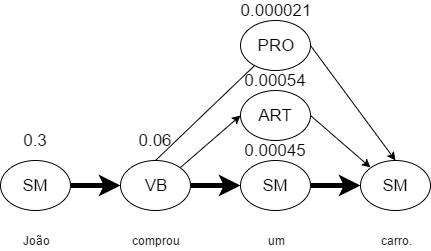
\includegraphics[height=180px]{imagens/markov2.png}
 \caption{Caminhos já decididos de classificação}
 \label{fig:markov2}
\end{figure}

Como visto, o método simbólico para resolver problemas de Processamento de
Linguagem Natural faz uso da criação de regras baseadas no conhecimento humano,
enquanto o método estatístico, decide através de cálculos probabilísticos
apoiados em estatísticas de um banco de dados para a resolução correta do
problema.


% Uma maneira de diferenciarmos os dois métodos é através do problema de
% ambiguidade. Por exemplo, nas frases:
% 
% ``João entrou no carro conversível de óculos novos.''. E ``João entrou no carro
% conversível de farol apagado.''.
% 
% Em ambas as frases, após a preposição ``de'' segue um substantivo masculino.
% Porém, cada uma das frases se refere a um substantivo diferente. A
% primeira se refere ao João, visto que não existe sentido em um carro ter óculos.
% Já a segunda se refere ao próprio carro, visto que não existe sentido em João
% ter faróis.
% 
% O método simbólico para resolver esse problema faz a criação de novas regras se
% baseadas no conhecimento humano para a solução de qual o significado da frase.
% Já o método estatístico, irá verificar qual a probabilidade de cada significado
% para cada frase através de análises similares decidindo através de metódos
% estatísticos qual o significado correto para cada frase
% \cite{jacksonmoulinier2007}.

\chapter{Métodos estatísticos e simbólicos aplicados na análise de sentimentos}
\label{cap:Classificadores}

%Para o \ac{NLP} e também para o campo de estatísticas, classificadores são
%algorítmos que identificam a qual categoria determinado item pertence. Essa
%classificação é feita a partir de dados já classificados corretamente, ou seja,
%um \textit{training set}.

\section{Naive Bayes}

O classificador Naive Bayes é um classificador baseado no teorema de Bayes com
independencia entre seus atributos.

O teorema de Bayes é representado da seguinte forma:

\[ P(c|d) = \frac{P(d|c) P(c)}{P(d)}  \]

Supondo que precisamos determinar se o carro que João comprou na frase ``João
comprou um Focus.'' é o modelo sedan ou hatch.
 
\begin{itemize}
  \item P(c$\vert$d) é a probabilidade de \textbf{d} pertencer a classe
  \textbf{c}. Ou seja, a probabilidade do carro Focus ser um sedan.
  \item P(d$\vert$c) é a probabilidade da classe \textbf{c} ser \textbf{d}. Ou
  seja, dentre todas as sedans, a probabilidade de um sedan ser
  um Focus.
  \item P(c) é a probabilidade da classe \textbf{c}. Ou seja, a frequência que
  sedans aparecem no nosso banco de dados.
  \item P(d) é a probabilidade de \textbf{d}. Ou seja, a frequência que Focus aparecem no nosso banco de dados.
\end{itemize}

Levando em consideração que temos o banco de dados representado pela tabela
abaixo:

\begin{table}[htb]
\centering
\label{123}
\begin{tabular}{|l|l|}
\hline
Carro  & Categoria \\ \hline
Focus  & Sedan     \\ \hline
Gol    & Hatch     \\ \hline
Focus  & Hatch     \\ \hline
Focus  & Sedan     \\ \hline
Focus  & Hatch     \\ \hline
Fox    & Hatch     \\ \hline
Fiesta & Hatch     \\ \hline
Cruze  & Sedan     \\ \hline
Focus  & Hatch     \\ \hline
\end{tabular} 
\caption{Tabela de Carro e Categoria.}
\end{table}

Probabilidade do Focus ser sedan:

\[ P(Sedan|Focus) = \frac{P(Focus|Sedan) P(Sedan)}{P(Focus)}  \]

\[ P(Sedan|Focus) = \frac{2/3 * 3/10}{5/10} = \frac{0,2}{0,5} = 0,4\]

Probabilidade do Focus ser um hatch:

\[ P(Hatch|Focus) = \frac{P(Focus|Hatch) P(Hatch)}{P(Focus)}  \]

\[ P(Hatch|Focus) = \frac{3/6 * 7/10}{5/10} = \frac{0,35}{0,5} = 0,7\]

No caso utilizado como exemplo, o Focus(Atributo ou \textit{Feature}) é um hatch
(Rótulo ou \textit{Label}).
Porém, caso tenhamos mais um atributo para utilizar na classificação o classificador Naive Bayes não
considera nenhuma dependência.
Como por exemplo a frase ``O carro era ano 2010 e tinha 2 portas'' com os
seguintes atributos:

\begin{table}[htb]
\centering
\begin{tabular}{|l|l|l|l|}
\hline
Carro  & Ano  & Portas & Categoria \\ \hline
Focus  & 2010 & 2      & Sedan     \\ \hline
Gol    & 2010 & 4      & Hatch     \\ \hline
Focus  & 2011 & 4      & Hatch     \\ \hline
Focus  & 2011 & 2      & Sedan     \\ \hline
Focus  & 2011 & 2      & Hatch     \\ \hline
Fox    & 2012 & 4      & Hatch     \\ \hline
Fiesta & 2012 & 2      & Hatch     \\ \hline
Cruze  & 2013 & 4      & Sedan     \\ \hline
Focus  & 2013 & 2      & Hatch     \\ \hline
\end{tabular}
\caption{Tabela de anos, carros, portas e categorias.}
\label{my-label}
\end{table}

O cálculo será feito da seguinte forma:

\[ P(d|c) = P(d_1|c) * P(d_2|c)* \ldots * P(d_n|c) \]

\[ P(Sedan|Focus) = P(Portas=2|Sedan) * P(Ano=2010|Sedan) \ldots * \]

\[ P(Sedan|Focus) = 2/3 * 1/3 \ldots * \]

Por assumir independência entre seus atributos, os valores obtidos nós cálculos
podem ser armazenados no banco de dados e reaproveitados. Por isso, sua
performance é considerada incrívelmente boa até mesmo para casos aonde temos forte dependência de
atributos \cite{domingos97naivebayes}.

%TODO EXEMPLO
\section{\textit{Maximum Entropy}}
O classificador \ac{MaxEnt} tem como
característica principal a preferência por modelos de dados uniformes sem efetuar nenhuma suposição injustificada.

Podemos utilizar um exemplo similar ao anterior para demonstrar a lógica do
classificador \ac{MaxEnt}. 
 
``João comprou um carro.''.

Supondo que temos que classificar o tipo de carro comprado em três categorias:

\begin{itemize}
  \item Hatch.
  \item Sedan.
  \item Cupê.
\end{itemize}

Podemos afirmar que:

\[ P(Hatch) + P (Sedan) + P(Cupe) = 1 \]

Como só temos essas três possibilidades de classificação no nosso
exemplo, o carro só pode ser classificado em uma dessas três possibilidades, ou
seja, a soma das três probabilidades deve ser 100\% ou 1 essa é a primeira
restrição ou \textit{constraint}. Abaixo duas tabelas que satisfazem essa
restrição:

\begin{table}[htb]
\centering
\begin{tabular}{|l|l|}
\hline
Tipo  & \%   \\ \hline
Sedan & 33\% \\ \hline
Hatch & 33\% \\ \hline
Cupê  & 33\% \\ \hline
 \end{tabular}
\caption{Tabela de Probabilidades A} 
\end{table}
\begin{table}[htb]
\centering
 \begin{tabular}{|l|l|}
\hline
Tipo  & \%   \\ \hline
Sedan & 50\% \\ \hline
Hatch & 50\% \\ \hline
Cupê  & 0\% \\ \hline
 \end{tabular}  
\caption{Tabela de Probabilidades B} 
\end{table}

Sem nenhum conhecimento prévio da distribuição desses carros, ou seja, a
quantidade de carros comprados por tipo, o classificador assume uma distribuição
uniforme das probabilidades, portanto, com maior entropia.

\begin{itemize}
  \item Hatch - 33\%.
  \item Sedan - 33\%.
  \item Cupê - 33\%.
\end{itemize}

Agora, supondo que a partir do nosso banco de dados conseguimos verificar que em
80\% dos casos o veículo comprado era um sedan ou hatch, temos uma nova
restrição:

\[ P(Hatch) + P (Sedan) = 0.8 \]

Podemos novamente ter n distribuições diferentes, porém a distribuição mais
uniforme que satisfaz as nossas duas restrições são:

\begin{itemize}
  \item Hatch - 40\%.
  \item Sedan - 40\%.
  \item Cupê - 30\%.
\end{itemize}

Esse é o princípio da Máxima Entropia utilizado nessa forma de classificação.
Primeiro é descoberta a frequência de cada atributo, depois é procurada a
distribuição que máximiza a entropia, ou seja, a mais uniforme.

%\subsection{Modelo Probabilístico}

%O seu modelo probabilístico para as probabilidades de observarmos o evento c
%quando d for verdadeiro:

%\[ P(c|d) := \frac{1}{Z(d)} exp (\Sigma_i\lambda_{i,c}F_{i,c}(d,c))\]





\section{\textit{VADER}}

O \ac{VADER} é um dicionário e classificador de sentimentos que se baseia em
regras, portanto, um método de classificação simbólico. Ele é especialmente
ajustado para funcionar em redes sociais aonde temos um contexto vago e pouca
quantidade de texto, nesse contexto, ele é extremamente eficaz, podendo se
comparar a classificação feita por humanos \cite{conf/icwsm/HuttoG14}.

Esse método faz uso de um dicionário que foi construído levando em consideração
gírias e emoticons utilizados em redes sociais. Neste dicionário as palavras
estão previamente associadas a uma polaridade de sentimento (positivo e
negativo) e intensidade em uma escala de -4 até +4, como por exemplo, a palavra
\textit{great} tem a intensidade de 3.1 e \textit{horrible} -2.5. Essa
associação foi construída utilizando o método de \textit{``wisdom of the
crowd''} aonde um grupo de pessoas atribuiu os valores para cada palavra ao
invés de somente uma pessoa especializada ou uma classificação automática
através de estatística.

Ele faz uso de cinco regras gerais:


\begin{itemize}
  \item Pontuação. O ponto de exclamação (!) aumenta a magnitude da
  intensidade sem modificar a orientação semântica. Como por exemplo,
  \textit{``This place is great!!!''} é mais intenso que \textit{``This place
  is great''}.
  \item Capitalização. Especificamente, uma palavra que é relevante para a
  análise de sentimentos, quando essa é escrita em letras maiúsculas, é
  aumentada a magnitude da intensidade do sentimento sem modificar a orientação
  semântica. Como por exemplo, na frase \textit{``This place is GREAT''}, temos
  a palavra \textit{``GREAT''} (Ótimo) que está relacionada com o sentimento
  positivo. Neste caso aonde ela está escrita em letras maiúsculas, ela é mais
  intensa que \textit{``This place is great''}.
  \item Advérbios intensificadores. Estes impactam a intensidade do sentimento
  aumentando ou diminuindo a intensidade do sentimento. Na frase \textit{``This
  place is extremelly good''} o advérbio \textit{extremelly} (extremamente)
  aumenta a intensidade do sentimento expresso pela frase (\textit{good} ou
  bom), enquanto na frase \textit{``This place is marginally good''}, a palavra
  \textit{``marginally'' ou marginalmente} acaba diminuindo a intensidade do
  sentimento expresso.
  \item A palavra \textit{``but''}. Essa palavra indica uma troca no sentimento
  da frase expressa aonde que o texto seguinte a ela expressa um sentimento mais
  dominante. Por exemplo, a frase \textit{``This place is great but today, the
  service was horrible''} convém um sentimento misto.
  \item Por fim, ao examinar as três palavras anteriores, o método consegue
  identificar 90\% dos casos aonde uma negação inverte a polaridade de um texto.
  Como por exemplo, na frase \textit{``This place isn't that great''}, a
  palavra \textit{great} demonstra um sentimento positivo, porém, ao analisar
  as três palavras anteriores \textit{``place isn't that''} encontramos uma
  negação, mudando o sentimento expresso da frase de positivo para negativo.
\end{itemize}

